\documentclass[8pt, xcolor={svgnames}]{beamer}
\usetheme[progressbar=frametitle]{metropolis}
\usepackage{appendixnumberbeamer}
\usepackage{url}
\usepackage{amsfonts} 
\usepackage{amssymb}
\usepackage[english]{babel}
\usepackage{fontawesome}
\usepackage{multicol}
\usepackage{bm}
\usepackage{braket}
\usepackage{algorithm}
\usepackage{algpseudocode}
\usepackage{enumitem}

\usepackage[]{pseudo}

\usepackage{tikz}
\usepackage[most]{tcolorbox}
\usepackage{xcolor}


\title{Density estimation via Quantum Adiabatic Machine Learning}
\date{Feb. 23, 2023}
\author[Matteo Robbiati]{Matteo Robbiati}



\begin{document}

\begin{frame}{Density estimation with adiabatic QML  \hfill \faBook\,\, \href{https://arxiv.org/abs/2303.11346}{arXiv:2303.11346}}
\small
\faCrosshairs\,\, Determining Probability Density Functions (PDF) by fitting the 
corresponding Cumulative Density Function (CDF) using an adiabatic QML ansatz.

\faFlash\,\, Algorithm's summary:
\begin{itemize}[noitemsep]
\item[1.] we optimize the parameters $\bm{\theta}$ of the following adiabatic evolution:
\begin{equation} 
H_{\rm ad}(\tau; \bm{\theta}) = [1-s(\tau; \bm{\theta})] \hat{X} + s(\tau; \bm{\theta})\hat{Z}
\end{equation}
in order to approximate some target CDF values with $\hat{F}(x_k \equiv \tau) = \braket{\psi(\tau)|\hat{Z}|\psi(\tau)}$;
\item[2.] we derivate from $H_{\rm ad}$ a circuit $\mathcal{C}(\tau; \bm{\theta})$ whose action 
on the GS of $\hat{X}$ returns $\ket{\psi(\tau)}$;
\item[3.] the circuit at step 2. can be used to calculate the CDF;
\item[4.] we compute the PDF by derivating $\mathcal{C}$ with respect to $\tau$ 
using the Parameter Shift Rule.
\end{itemize}
\begin{figure}  
    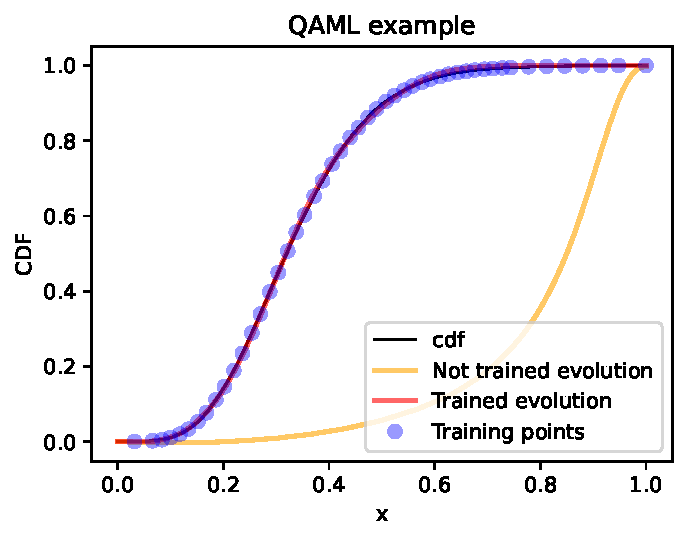
\includegraphics[width=0.5\textwidth]{figures/evolution.pdf}%
    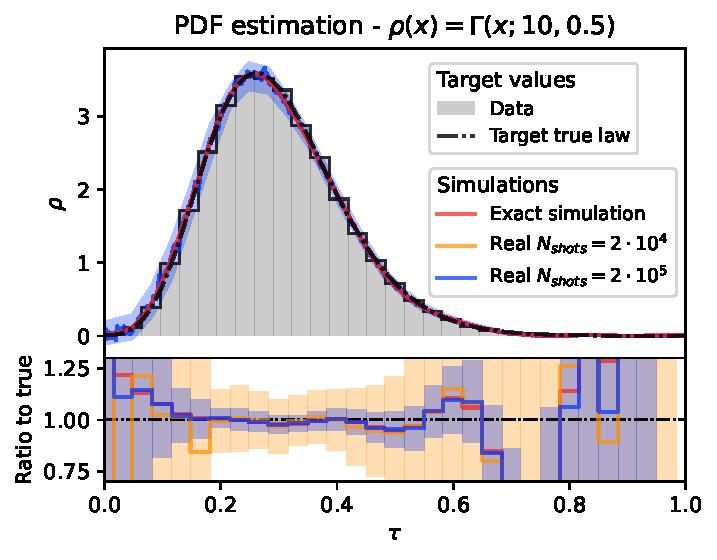
\includegraphics[width=0.5\textwidth]{figures/PDF.pdf}
\end{figure}


\end{frame}

\begin{frame}{Multi-variable integration with VQCs \hfill \faBook\,\, \href{https://arxiv.org/abs/2308.05657}{arXiv:2308.05657}}
\small
\faCrosshairs\,\, Use Variational Quantum Circuits to calculate multi-dimensional 
integrals of the form:
\begin{equation}
I(\alpha) = \int_{\bm{x}_a}^{\bm{x}_b} g(\alpha; \bm{x}) \text{d}^n \bm{x}.
\label{eq:integral}
\end{equation}

\faFlash\,\, Algorithm's summary:

\begin{itemize}[noitemsep]
\item[1.] inspired by \href{https://arxiv.org/abs/2211.02834}{arXiv:2211.02834}, 
we train the derivative of a VQC with respect to the integral variables $\bm{x}$ to approximate 
the integrand $g(\bm{x})$;
\item[2.] the derivatives are computed using the Parameter Shift Rule and this
allows the same circuit $\mathcal{C}$ to be used for approximating any integrand 
marginalisation and the primitive!
\item[3.] thanks to 2., it's much more convenient to compute Eq.~\eqref{eq:integral}
when varying $\alpha$.
\end{itemize}
\begin{figure}  
    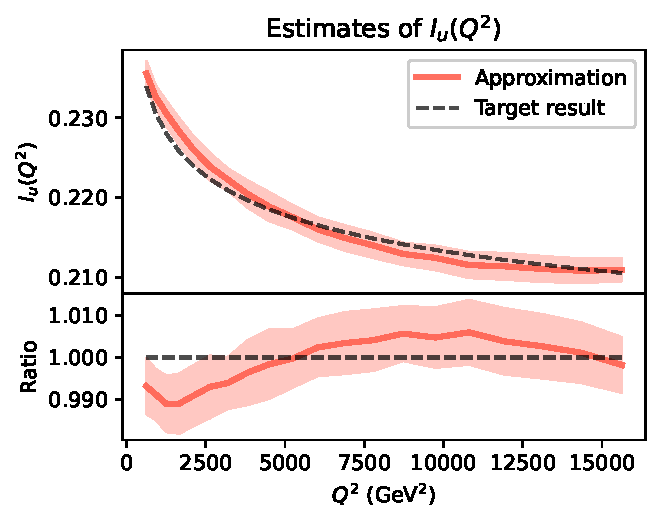
\includegraphics[width=0.5\textwidth]{figures/uquark2d.pdf}%
    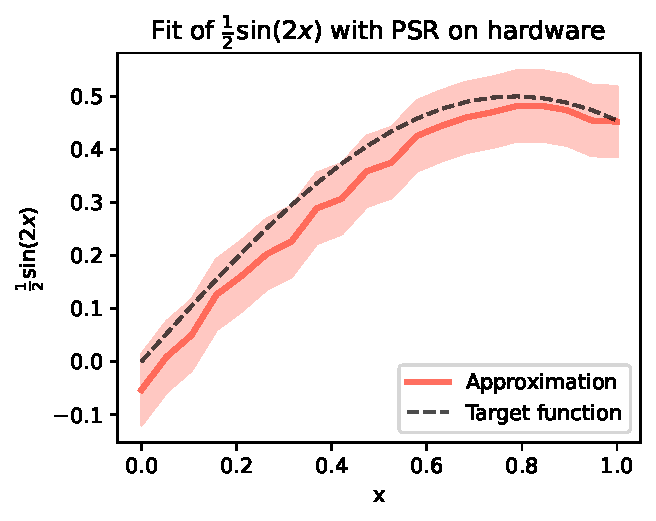
\includegraphics[width=0.5\textwidth]{figures/hardware_int.pdf}
\end{figure}
\end{frame}

\begin{frame}{Real time error mitigation in QML trainings \hfill \faBook\,\, Coming soon!}
\small
\faCrosshairs\,\, Cleaning up the parameters space with a real time error mitigation
strategy in order to overcome Noise-Induced Barren Plateaus (NIBP) when training 
a QML model.

\faFlash\,\, Algorithm's summary:

\begin{itemize}[noitemsep]
\item[1.] we mitigate all the expected values $E$ through Clifford Data Regression (CDR):
\begin{equation}
E_{\rm mit} = \alpha_{\rm cdr} E_{\rm noisy} + \beta_{\rm cdr};
\end{equation}
\item[2.] reduced CDR computational cost by updating $(\alpha, \beta)_{\rm cdr}$
periodically during the training;
\item[3.] the mitigation removes the bounds and accelerate the training process.
\end{itemize}
\begin{figure}  
    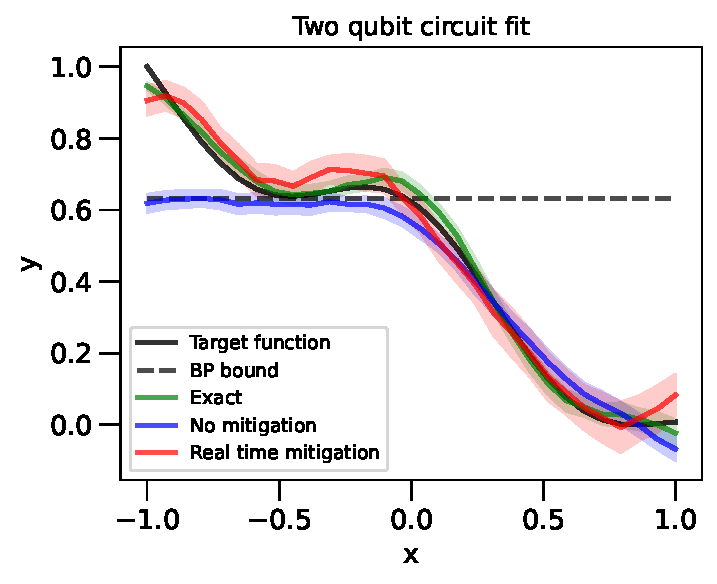
\includegraphics[width=0.5\textwidth]{figures/fits_benchmark.pdf}%
    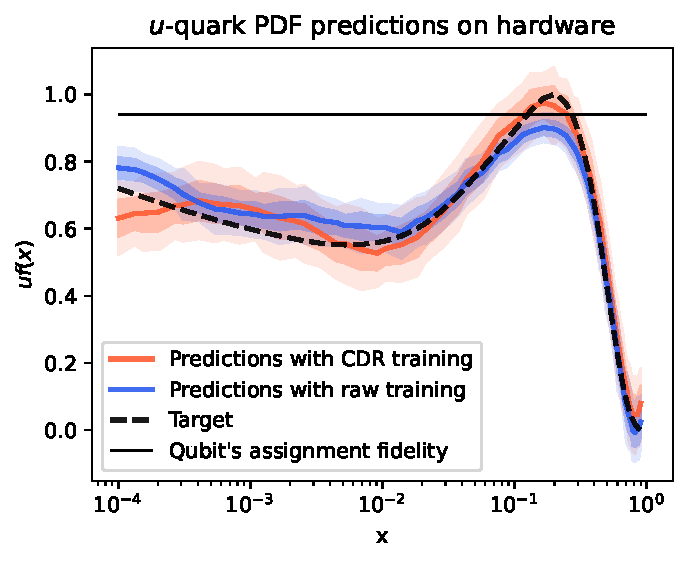
\includegraphics[width=0.5\textwidth]{figures/hardware.pdf}
\end{figure}
\end{frame}

\end{document}
